\documentclass[aspectratio=169]{beamer}
\usepackage[utf8]{inputenc}
\usepackage[T1]{fontenc}

\usetheme{focus}
\definecolor{main}{RGB}{11, 93, 25}

\usecolortheme[RGB={11,93,20}]{structure}
\usepackage[spanish]{babel}

\usepackage{colortbl}
\usepackage{color}
\usepackage{pifont}
\usepackage{ulem}



\usepackage{colortbl}
\usepackage{color}
\usepackage{pifont}
% \usepackage[normalem]{ulem}                                                                                                                                
\usepackage{hyperref}
\hypersetup{
    colorlinks=true,
    linkcolor=blue,
    filecolor=magenta,
    urlcolor=cyan,
}

\usepackage{listings}

\parskip=12pt

\lstset{basicstyle=\normalsize,
aboveskip=5pt,
basicstyle=\small\ttfamily,
belowskip=5pt
}

\author{Alberto Molina Coballes\\
José Domingo Muñoz Rodríguez}
\title{Introducción a docker}
\institute{IES Gonzalo Nazareno}
\titlegraphic{
\includegraphics[width=1.5cm]{cc_by_sa.png}}
\logo{
\includegraphics[width=.75cm]{logo_iesgn.png}}
\date{\today}

\definecolor{verde}{rgb}{0,0.73,0}

\begin{document}
\begin{frame}[t,plain]
\titlepage
\end{frame}

\begin{frame}
  \frametitle{Docker}
  \begin{itemize}
  \item “docker”: estibador
  \item Pertenece a los denominados contenedores de aplicaciones
  \item Gestiona contenedores a alto nivel proporcionando todas las capas y funcionalidad adicional
  \item Nuevo paradigma. Cambia completamente la forma de desplegar y distribuir una aplicación
  \item Docker: build, ship and run
  \item Lo desarrolla la empresa Docker, Inc.
  \item Instalación y gestión de contenedores simple
  \item El contenedor ejecuta un comando y se para cuando éste termina, no es un sistema operativo al uso, ni pretende serlo
  \item Escrito en go
  \item Software libre (ha ido cambiando con el tiempo)
  \end{itemize}
\end{frame}

\begin{frame}
  \frametitle{Docker}
  \begin{columns}
    \column{0.7\textwidth}
    \begin{itemize}
    \item docker engine
      \begin{itemize}
      \item demonio docker
      \item docker API
      \item docker CLI
      \end{itemize}
    \item docker-machine
      \begin{itemize}
      \item Gestiona múltiples docker engine
      \end{itemize}
    \item docker compose
      \begin{itemize}
      \item Para definir aplicaciones que corren en múltiples contenedores
      \item Ejemplo: \href{https://github.com/bitnami/bitnami-docker-wordpress/blob/master/docker-compose.yml}{docker-compose.yml}
      \end{itemize}
      \item docker swarm
        \begin{itemize}
        \item Orquestador de contenedores
        \end{itemize}
      \end{itemize}
      \column{0.3\textwidth}
      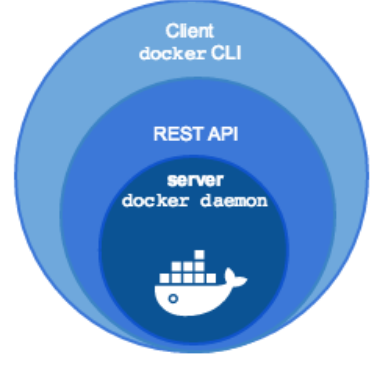
\includegraphics[width=\textwidth]{img/docker-engine.png}
  \end{columns}
\end{frame}

\begin{frame}
  \frametitle{Docker. Evolución del proyecto}
  \begin{itemize}
  \item El dilema de docker inc. entre el éxito y el negocio
  \item OCI: Open Containers Initiative
  \item runtime-spec: \url{http://www.github.com/opencontainers/runtime-spec}
  \item image-spec: \url{http://www.github.com/opencontainers/image-spec}
  \item distribution-spec: \url{https://github.com/opencontainers/distribution-spec}
  \item El cambio en docker
    \begin{itemize}
    \item Moby (proyecto de comunidad) (docker.io de debian)
    \item docker CE (docker engine proporcionado por Docker inc)
    \item docker EE (docker engine + servicios de Docker inc)
    \item runc (OCI) \url{https://github.com/opencontainers/runc}
    \item containerd (CNCF) \url{https://github.com/containerd/containerd}
    \end{itemize}
  \end{itemize}
\end{frame}

\begin{frame}
  \frametitle{Docker. Componentes}
  \begin{center}
  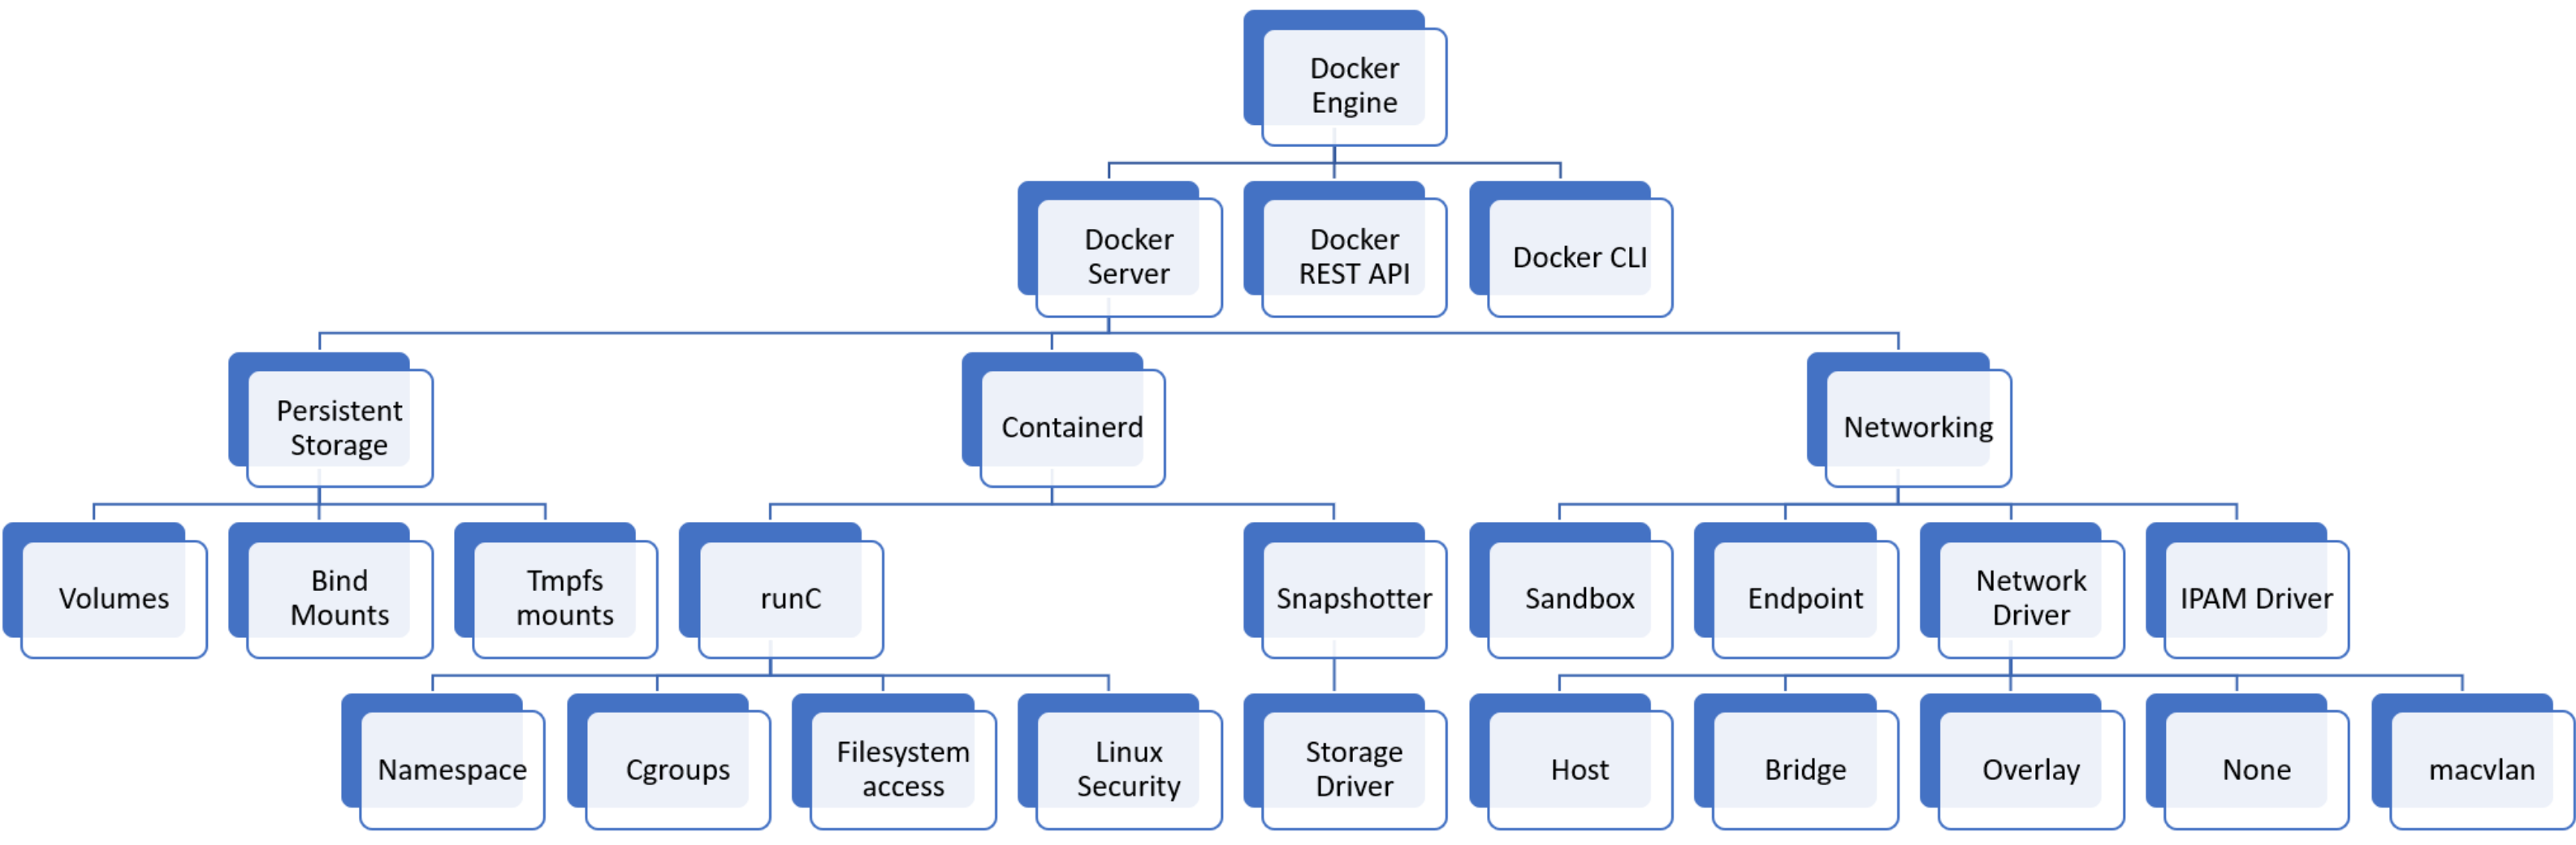
\includegraphics[width=.7\textwidth]{img/componentes-docker.png}
  \end{center}
  \begin{itemize}
  \item Si vamos a utilizar un orquestador diferente a docker swarm,
    ¿necesitamos docker engine o containerd?
  \item runc es equivalente a lxc
  \item runc y containerd son proyectos de software libre independientes de docker
  \end{itemize}
\end{frame}

\begin{frame}
  \frametitle{Alternativas a docker}
  \begin{description}
  \item [rkt] inicialmente desarrollado por CoreOS. Actualmente dentro
    de la Cloud Native Computing Foundation:
    \url{https://github.com/rkt/rkt} y enfocado a ser una alternativa
    a containerd
  \item[cri-o] Creado por Red Hat como alternativa a containerd y pensado solo para funcionar integrado en kubernetes \url{https://cri-o.io/}
  \item[podman] Creado por Red Hat como alternativa a docker
    \url{https://podman.io}
  \item[pouch] Creado por Alibaba como alternativa a
    docker. \url{https://pouchcontainer.io}
  \item[kata] MVs ligeras para para proporcionar mayor aislamiento.
    \url{https://katacontainers.io/}
  \item[nemu] \url{https://github.com/intel/nemu}
  \item[firecracker] Desarrollado por AWS \url{https://github.com/firecracker-microvm/firecracker}
  \end{description}
\end{frame}

\end{document}
